\section{Introduction to Dynamic Programming}

\begin{frame}
  \begin{center}
    {\bf Part I -- Introduction}
  \end{center}
\end{frame}

\subsection{Definitions}
\begin{frame}
  \frametitle{What is Dynamic Programming (DP)?}

  \structure{DP} is a \structure{Search Algorithm} based on the idea of {\bf Storing Partial Solutions in Memory}.

  \bigskip

  \begin{block}{Basic Idea of DP}
    \begin{itemize}
      \item Create a {\bf DP table}. The dimensions are the parameters of a recursive function that generates the solution to the problem; \bigskip

      \item First fill in the table with the starting conditions;\bigskip

      \item Next use the recursive function (or a for loop) to fill the rest of the table;\bigskip

      \item Find the answer;
    \end{itemize}
  \end{block}
\end{frame}

\begin{frame}{What is Dynamic Programming (DP)?}{Characteristics}

  \begin{block}{If a problem requires {\bf optimization} or {\bf counting}, then it "smells of DP"}

    \begin{itemize}
    \item ``Count the number of solutions...''
    \item ``Find the minimum cost...''
    \item ``Find the maximum length...''
    \end{itemize}
  \end{block}

  \begin{exampleblock}{What is the running cost of DP?}
    The algorithm evaluates each element of the DP table.\medskip

    So the cost of a DP algorithm is proportional to the {\bf size of the DP table.}
  \end{exampleblock}

  You can prove a DP algorithm to be correct using {\bf Proof by Induction}.
\end{frame}

\subsection{Example Problem I}

\begin{frame}{Problem Example: Wedding Shopping}{Problem Summary}

  We have to choose a set of items to buy, within a maximum budget $M$.

    \begin{columns}
      \column{0.7\textwidth}
    \begin{itemize}
      \item There are $C$ classes of items;
      \item Each class has $K_c$ options;
      \item Each option ($K_{c,i}$) has a different cost;
      \bigskip

      \item Buy one item from each Class;
      \item Maximize the total cost, but {\bf do not} exceed the budget $M$;
      \bigskip

      \item Limits: $M \leq 200$, $1 < C \leq 20$, $0 < K_c \leq 20$
    \end{itemize}

      \column{0.3\textwidth}
      \includegraphics[width=.8\textwidth]{../img/weddingdress}\\
    \end{columns}\bigskip

    {\bf QUIZ: How many possible combinations exist in the largest case?}

    \ppagenote{Wedding Dress Image CC-By-2.0 by \url{https://www.flickr.com/photos/vancouver125/5634967507}}
\end{frame}

\begin{frame}{Problem Example: Wedding Shopping}{Solution Example}
  \begin{block}{Sample case 1: $C=3, K_c = \{3,2,4\}$}
  \begin{tabular}{|c|cccc|}
    Class & 1 & 2 & 3 & 4\\
    \hline
    $K_0$ & 6 & 4 & 8 & \\
    $K_1$ & 5 & 10 & & \\
    $K_2$ & 1 & 5 & 3 & 5\\
  \end{tabular}
  \end{block}
  \medskip

  If the budget is $M=20$, the answer is $19$. Three ways to reach this answer:
  \begin{itemize}
    \item $8(K_{0,2})+10(K_{1,1})+1(K_{2,0})$
    \item $6(K_{0,0})+10(K_{1,1})+3(K_{2,2})$
    \item $4(K_{0,1})+10(K_{1,1})+5(K_{2,1} \text{ or } K_{2,3})$
  \end{itemize}
  \bigskip

  However, if the budget is $M=9$, There is no solution for the problem.\\
  Because the minimum possible cost is $10$, or $4(K_{0,1})+5(K_{1,0})+1(K_{2,0})$
\end{frame}

\begin{frame}[fragile]{Problem Example: Wedding Shopping}{Complete Search Solution}
  This is a {\bf Search problem}: one solution is defined as "one choice from each class".\medskip

  Unfortunately, a Greedy Algorithm will not work in this algorith. So first let's describe a full recursive search:


{\smaller
\begin{verbatim}
shop(m,g):                 // Recursive function. Returns the money used
                           // after start buying from category "g"
  if (m > M) return -1     // End case -- we spend more money than the budget.
  if (g == C) return m     // End case -- we bought all categories.
                           //             Return the total money used.
  for each i in Kc:
    totals[i] = shop(m + price[g][i], g+1) // try buying item i at category g.

  return max(totals)       // Return the value of the best item.

shop(0,0)                  // Start condition: buying from category 0
                           // No money used.
\end{verbatim}
}
\end{frame}

\begin{frame}{Problem Example: Wedding Shopping}{Complete Search Solution -- Time Limited Exceeded :-(}

  In the worst case, there are a total of $20^{20}$ possible choices. So the complete solution will not solve this problem...\bigskip

  \begin{block}{Problem: Too many overlapping subproblems}
    \medskip
    \begin{columns}[T]
      \column{0.4\textwidth}
      \hspace{.5cm}\begin{tabular}{|c|cccc|}
        Class & 1 & 2 & 3 & 4\\
        \hline
        0 & 6 & 4 & 8 & 12\\
        1 & 4 & 6 & 6 & 2\\
        2 & 1 & 5 & 1 & 5\\
        3 & 2 & 4 & 6 & 2\\
      \end{tabular}

      \column{0.6\textwidth}
      Consider: How many times the program in the last slide will call "\emph{shop(10,2)}?"\medskip

      \begin{itemize}
        \item shop(0,0) $\to$ shop(6,1) $\to$ shop(10,2)
        \item shop(0,0) $\to$ shop(4,1) $\to$ shop(10,2) x2
        \item shop(0,0) $\to$ shop(8,1) $\to$ shop(10,2)
      \end{itemize}\medskip

      Every time \emph{shop(10,2)} is called, {\bf the return value is always the same.}
    \end{columns}
  \end{block}
\end{frame}


\begin{frame}
  \frametitle{Wedding Shopping -- the DP approach}

  When a problem has this characteristic ({\bf repeated sub-structures}), it is a strong hint that DP is a good solution.
  \bigskip

  First, we create a {\bf DP table} using the parameters of the "shop(m,g)" function.\bigskip

  Remember: "shop(m,g)" always returns the same value.

  \begin{block}{How big is the table?}
    The table stores all possible calls of \emph{shop(m,g)}, so the table size is $|M| \times |C|$.
    \bigskip

    Remember that $0 \leq M \leq 200$ and $1 < C \leq 20$, so our table has \alert{$201*20=4020$ states}.
  \end{block}
  \smallskip

  That is a very small number! This algorithm will be FAST, compared to $20^{20}$.
\end{frame}

\begin{frame}{Wedding Shopping -- the DP approach}{How to fill the table?}

  There are two main approaches for filling the {\bf DP table}:
  \bigskip

  \begin{itemize}
  \item {\bf Top-down approach}: \\Use the DP table as a "memory" table.\\
  Every time we call the function: If the result is in the table, use that result. If not, calculate and store in the table. Very common with {\bf "recursive functions"}.
  \vfill

  \item {\bf Bottom-up approach}: \\
  First we complete the starting values of the table. Then we fill other values based on the starting values. Very common with {\bf "for loops"}.
  \end{itemize}
\end{frame}

%%%%%%%%%%%%%%
%% Solution: Dynamic Programming
% Programming here is not "code", but a "tabular method" (table method)

%% DP us normally used when
% Program has optimal sub structure:
%   The optimal solution to the problem contain optimal solutions to sub problems
%   - "similar" to the requirement of greedy
%   - If you can make a complete search recurrent (recursive), then you have this
% The subproblems are overlapping
%   - The number of _Distinct_ subproblems is small, but they are computed repeatedly
%   - Different from divide and conquer, in DC the sub problems are distinct
%%%%%%%%%%%%%
\subsection{DP Programming Examples}

\begin{frame}[fragile]{Wedding Shopping -- the DP approach}
  {Using Top-down DP -- very easy to program!}

\begin{block}{}
{\smaller
\begin{verbatim}
memset(table, -2, sizeof(table))  //-1 = "no result", -2 = "not visited"

shop(m,g):
  if (m > M) return -1                      // End States are the same;
  if (g == C) return m
  if (table[m][g] != -2) return table[m][g] // Check if the result is in memory

  for each i in Kc:                         // Calculate as before;
    totals[i] = shop(m + price[g][i], g+1)

  table[m][g] = max(totals)                 // Store new result in table;
  return table[m][g]

shop(0,0)                                   // That's the only change!
\end{verbatim}}
\end{block}
\end{frame}

%%% TODO: Add how to print after the bottom up DP
%% What if you need to print the result (maybe not add this?)
% for each level, you check the lower level to see which one matches the current state
% See slide 16 for details

\begin{frame}{Wedding Shopping -- The DP approach}{Using bottom-up DP}
  Algorithm:
  \begin{itemize}
  \item Prepare a table with the problem states (same table as top-down);
  \item Choose the initial states of the table;
  \item Mark the initial states as "unprocessed";
  \item {\bf (Loop)} For each unprocessed value, calculate its value, and add the new unprocessed values.
  \end{itemize}

  \vfill

  The main difficulties in bottom-up DP are:
  \begin{itemize}
    \item To find the initial states;
    \item To choose the processing function;
  \end{itemize}
  After that, it is just a big "for loop".
\end{frame}

\begin{frame}{Wedding Shopping -- Bottom-up DP}{One possible solution}

  Example: M=10, \alert<2>{$K_0=\{2,4\}$}, \alert<3>{$K_1=\{4,6\}$}, \alert<4>{$K_2=\{1,3,2,1\}$}
  \bigskip

  \begin{tabular}{|c||c|c|c|c|c|c|c|c|c|c|c|c|}
    \hline
    M & 0 & 1 & 2 & 3 & 4 & 5 & 6 & 7 & 8 & 9 & 10\\
    \hline
    $g=0$ & X & & & & & & & & & & \\
    $g=1$ & & & \only<2->{X} & & \only<2->{X} & & & & & & \\
    $g=2$ & & & & & & & \only<3->{X} & & \only<3->{X} & & \only<3->{X}\\
    $g=3$ & & & & & & & & \only<4->{X} & \only<4->{X} & \only<4->{X} & \only<4->{X}\\
    \hline
  \end{tabular}

  \begin{itemize}
  \item {\bf Start state}: We use no money, so mark $T(0,0)$ as "unprocessed".
  \item {\bf Transition Function} (from category c to category c+1):
    \begin{itemize}
      \item Loop on money: $i = 0\to m$
      \item If $T(g,i)$ is marked as "unprocessed"
      \begin{itemize}
        \item Loop: $j = 0\to |K_c|$
        \item Mark $T(s+1,i+K_{c,j})$ as "unprocessed"
      \end{itemize}
    \end{itemize}
  \item {\bf Solution}: The solution is the maximum column marked when $g = C$
  \end{itemize}
\end{frame}

\begin{frame}[fragile]{Wedding Shopping -- Bottom-up DP}

  Example: M=10, $K_0=\{2,4\}$, $K_1=\{4,6\}$, $K_2=\{1,3,2,1\}$
  \bigskip

  \begin{tabular}{|c||c|c|c|c|c|c|c|c|c|c|c|c|}
    \hline
    M & 0 & 1 & 2 & 3 & 4 & 5 & 6 & 7 & 8 & 9 & 10\\
    \hline
    $s=0$ & X & & & & & & & & & & \\
    $s=1$ & & & X & & X & & & & & & \\
    $s=2$ & & & & & & & X & & X & & X\\
    $s=3$ & & & & & & & & X & X & X & X\\
    \hline
  \end{tabular}
  {\smaller
  \begin{block}{}
\begin{verbatim}
memset(table,0,sizeof(table))
table[0][0] = 1

for g in (0 to C-1)
  for i in (0 to M-1):
    if table[g][i] == 1:
       for k in (0 to K[g]-1):
          table[g + 1][i + cost[g][k]] = 1 // Don't forget out of bounds check!
\end{verbatim}
  \end{block}}
\end{frame}

\begin{frame}
  \frametitle{DP: Top-down or Bottom-up?}

  \begin{block}{Top-Down}
    {\bf Pros:} Easy to implement, just add memory to a recursive search. Only computes the visited states of the DP table. \medskip

    {\bf Cons:} Overhead of recursive function. Hard to reduce the size of the DP table.
  \end{block}

  \begin{block}{Bottom-Up}
    {\bf Pros:} Faster if you will visit the entire DP table anyway. It is possible to save memory by discarding old rows.\medskip

    {\bf Cons:} Harder to think the algorithm. If the DP table is sparse, the loop will visit every state.
  \end{block}
\end{frame}

\subsection{DP Example 2}

\begin{frame}{Finding the Decision Set with DP}

  In the example we studied, the program only returns the total money used.\bigskip

  In some problems, we also need to output the {\bf optimal solution} (for example, optimal path). How do we do that?
  \bigskip

  It is not very hard. You need TWO tables:
  \begin{itemize}
    \item Table 1: The DP table (memory table);
    \item Table 2: The "Parent" table, which indicate what was the previous choice.
  \end{itemize}
  \bigskip

  The next example will show the use of the "Parent" table. \bigskip

  \begin{block}{}
    When filling the parent table, be careful about the rules for tie breaking!\\
    (Lexographical order, smallest solution, etc).
  \end{block}
\end{frame}

\begin{frame}{Example 2: Apple Field}
  \begin{block}{}
  {\smaller
  A farmer has an apple field, and a robot to collect the apples. However, the robot can only move {\bf one left} or {\bf one down}. The robot starts at position $(0,0)$, and ends at $(n,n)$.\medskip

  You know how many apples are in each cell. What is the path with maximum apples?
}
  \end{block}

  \begin{center}
    \includegraphics[width=0.4\textwidth]{../img/applefield}
  \end{center}
\end{frame}

\begin{frame}{Example 2: Apple Field}{One Possible Solution (Not maximum)}

  \begin{columns}
    \column{0.5\textwidth}
    L, D, L, L, L, L, L, L, D, D, D, D, L, D
    \column{0.5\textwidth}
    \includegraphics[width=0.9\textwidth]{../img/applefield-solution}
  \end{columns}
\end{frame}

\begin{frame}{Example 2: Apple Field}{Complete Search}

  \begin{block}{}
    How many different paths are possible?
  \end{block}
  \begin{itemize}
    \item A path has $n$ steps left (0), and $n$ steps down (1), in any order.
    \bigskip

    \item A path is a string with size $2n$, $n$ "0"s, and $n$ "1"s.
    \bigskip

    \item Permutation of $2n$ with $n$ "0"s and $n$ "1"s: $\binom{2n}{n} = \frac{(2n)!}{n!n!}$
    \begin{itemize}
      \item Too big for full search!
    \end{itemize}
  \end{itemize}\bigskip

  Like in the "Wedding Shopping" problem, we have {\bf overlapping subproblems}.
  \bigskip

  For example, the optimal path from $(x,y)$ to $(n,n)$ is always the same, regardless of the path from $(0,0)$ to $(x,y)$. So let's try DP!
\end{frame}


\begin{frame}{Example 2: Apple Field}{Bottom-up DP}
  \begin{itemize}
  \item {\bf DP table and Parent table:}
  \begin{itemize}
    \item The DP table is a $n+1\times n+1$ table. At every position, we have the maximum number of apples from $(0,0)\to(x,y)$.
    \item The Parent table is a $n+1\times n+1$ table. At every position, we store the last-1 cell (up or right) of $(0,0)\to(x,y)$.
  \end{itemize}

  \item {\bf Initial Condition:} (DP table only)
  \begin{itemize}
    \item To avoid special treatment of the first row and first column, we include a "boundary" at the top and right of the table. Every cell at the boundary has "0" apples
  \end{itemize}

  \item {\bf Transition:}
  \begin{itemize}
    \item We double loop over the DP table (row $\to$ column, or vice-versa). For every cell $(x,y)$:\\
    $DP[x][y] = \text{apple}[x][y] + \text{max}(DP[x-1][y],DP[x][y-1])$\\
    $\text{Parent}[x][y] = (DP[x-1][y] > DP[x][y-1]?\leftarrow:\uparrow)$
  \end{itemize}
  \end{itemize}
\end{frame}

\begin{frame}[fragile]{Example 2: Apple Field}{Pseudocode}
  {\smaller
  \begin{block}{}
\begin{verbatim}
int apple[m+1][n+1];     // Input Data. Board index is from 1 to n

int DP[m+1][n+1];                      // DP Table
DP[0][0..n+1] and DP[0..m+1][0] = 0;   // Initial states;

int parent[m+1][n+1];               // Parent Table;

for (int i = 1; i < m+1; i++) {
  for (int j = 1; j < n+1; j++) {
    DP[m][n] = apple[m][n] + max(DP[m][n-1], DP[m-1][n]);  // Update DP
    if (DP[m][n-1] > DP[m-1][n]):                          // Update Parent
       parent[m][n] = "left";
    else:
       parent[m][n] = "up";
  }
}
\end{verbatim}
\end{block}
  }
\end{frame}



\begin{frame}[fragile]{Example 2: Apple Field}{Simulating the algorithm}

{\smaller
\begin{verbatim}
DP[m][n] = apple[m][n] + max(DP[m][n-1], DP[m-1][n]);
if (DP[m][n-1] > DP[m-1][n]):
   parent[m][n] = "left";
else:
   parent[m][n] = "up";
 \end{verbatim}}

\begin{columns}
  \column{0.3\textwidth}
  \begin{center}
    Input Table\\
    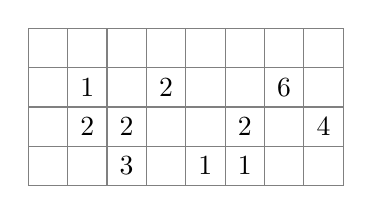
\begin{tikzpicture}
    \draw[step=0.5cm,color=gray] (0,0) grid (4,2);
    %% Row 1
    \node at (.75,1.25) {1};
    \node at (1.75,1.25) {2};
    \node at (3.25,1.25) {6};
    %% Row 2
    \node at (.75,.75) {2};
    \node at (1.25,.75) {2};
    \node at (2.75,.75) {2};
    \node at (3.75,.75) {4};
    %% Row 3
    \node at (1.25,.25) {3};
    \node at (2.25,.25) {1};
    \node at (2.75,.25) {1};
    \end{tikzpicture}
  \end{center}

  \column{0.3\textwidth}
  \begin{center}
  DP Table\\
    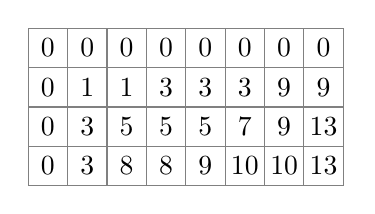
\begin{tikzpicture}
    \draw[step=0.5cm,color=gray] (0,0) grid (4,2);
    \node at (.25,.25) {0};
    \node at (.25,.75) {0};
    \node at (.25,1.25) {0};
    \node at (.25,1.75) {0};
    %
    \node at (.75,1.75) {0};
    \node at (1.25,1.75) {0};
    \node at (1.75,1.75) {0};
    \node at (2.25,1.75) {0};
    \node at (2.75,1.75) {0};
    \node at (3.25,1.75) {0};
    \node at (3.75,1.75) {0};
    %
    \node<2-> at (.75,1.25) {1};
    \node<3-> at (1.25,1.25) {1};
    \node<4-> at (1.75,1.25) {3};
    \node<5-> at (2.25,1.25) {3};
    \node<5-> at (2.75,1.25) {3};
    \node<6-> at (3.25,1.25) {9};
    \node<6-> at (3.75,1.25) {9};
    %
    \node<7-> at (.75,.75) {3};
    \node<8-> at (1.25,.75) {5};
    \node<9-> at (1.75,.75) {5};
    \node<9-> at (2.25,.75) {5};
    \node<10-> at (2.75,.75) {7};
    \node<11-> at (3.25,.75) {9};
    \node<12-> at (3.75,.75) {13};
    %
    \node<13-> at (.75,.25) {3};
    \node<13-> at (1.25,.25) {8};
    \node<13-> at (1.75,.25) {8};
    \node<13-> at (2.25,.25) {9};
    \node<13-> at (2.75,.25) {10};
    \node<13-> at (3.25,.25) {10};
    \node<13-> at (3.75,.25) {13};
    \end{tikzpicture}
  \end{center}

  \column{0.3\textwidth}
  \begin{center}
  Parent Table\\
    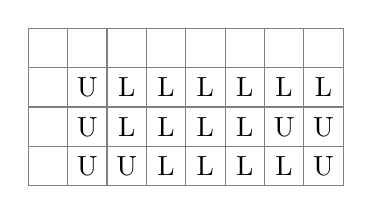
\begin{tikzpicture}
    \draw[step=0.5cm,color=gray] (0,0) grid (4,2);
    %\node at (.25,1.25) {0};
    \node<2-> at (.75,1.25) {U};
    \node<3-> at (1.25,1.25) {L};
    \node<4-> at (1.75,1.25) {L};
    \node<5-> at (2.25,1.25) {L};
    \node<5-> at (2.75,1.25) {L};
    \node<6-> at (3.25,1.25) {L};
    \node<6-> at (3.75,1.25) {L};
    %
    \node<7-> at (.75,.75) {U};
    \node<8-> at (1.25,.75) {L};
    \node<9-> at (1.75,.75) {L};
    \node<9-> at (2.25,.75) {L};
    \node<10-> at (2.75,.75) {L};
    \node<11-> at (3.25,.75) {U};
    \node<12-> at (3.75,.75) {U};
    %
    \node<13-> at (.75,.25) {U};
    \node<13-> at (1.25,.25) {U};
    \node<13-> at (1.75,.25) {L};
    \node<13-> at (2.25,.25) {L};
    \node<13-> at (2.75,.25) {L};
    \node<13-> at (3.25,.25) {L};
    \node<13-> at (3.75,.25) {U};
    \end{tikzpicture}
  \end{center}
\end{columns}

\end{frame}
